\documentclass[tikz,border=5pt]{standalone}
\begin{document}
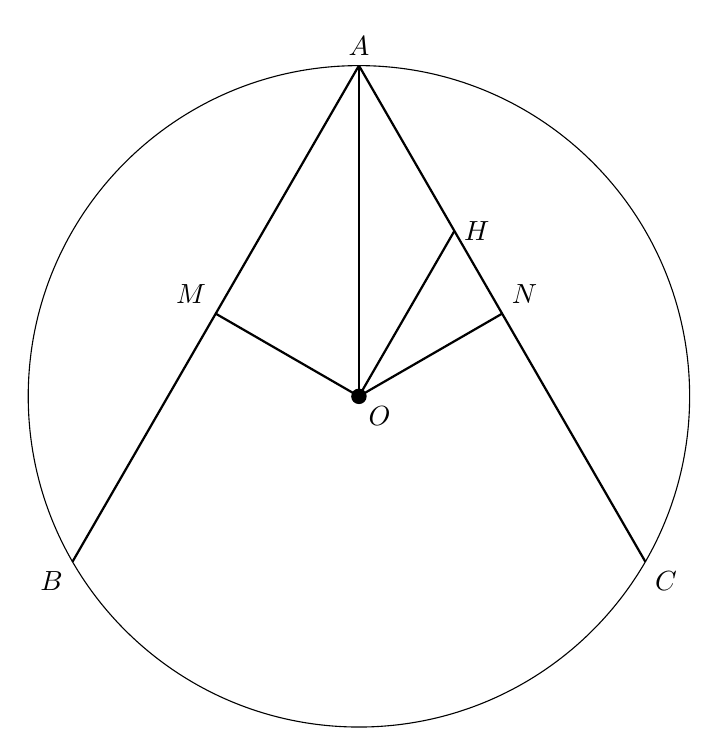
\begin{tikzpicture}[scale=1.4]
  % 圆
  \draw (0,0) circle (3);
  % 主要点
  \coordinate (A) at (0,3);
  \coordinate (B) at (-2.598,-1.5);
  \coordinate (C) at (2.598,-1.5);
  \coordinate (O) at (0,0);
  \coordinate (M) at (-1.299,0.75);
  \coordinate (N) at (1.299,0.75);
  \coordinate (H) at (0.866,1.5);
  % 线段
  \draw[thick] (A) -- (B);
  \draw[thick] (A) -- (C);
  \draw[thick] (A) -- (O);
  \draw[thick] (O) -- (M);
  \draw[thick] (O) -- (N);
  \draw[thick] (O) -- (H);
  % 点 O
  \fill (O) circle (2pt);
  % 标签
  \node[above] at (A) {$A$};
  \node[below left] at (B) {$B$};
  \node[below right] at (C) {$C$};
  \node[above left] at (M) {$M$};
  \node[above right] at (N) {$N$};
  \node[below right] at (O) {$O$};
  \node[right] at (H) {$H$};
\end{tikzpicture}
\end{document}
